% No New page; first instance
\visHeader

Our EA extension provides rudimentary support for validating the static semantics (Ecore) and dynamic semantics (SDM) of metamodels.
Validation results are displayed and, in some cases, even ``quick fixes'' to automatically solve the problems are offered.
Our validation framework is still work in progress so if you find an error that is not/wrongly detected feel free to send us a brief description.

\begin{enumerate}
\item[$\blacktriangleright$] To make the validation output window visible in EA, choose ``Extensions/\-Add-In Windows''.
This should display a new output window as depicted in Fig.~\ref{fig:validation_output}. This control panel also contains shortcuts for all the functionality available via the extensions file menu and many users actually prefer this.

\begin{figure}[htbp]
	\centering
  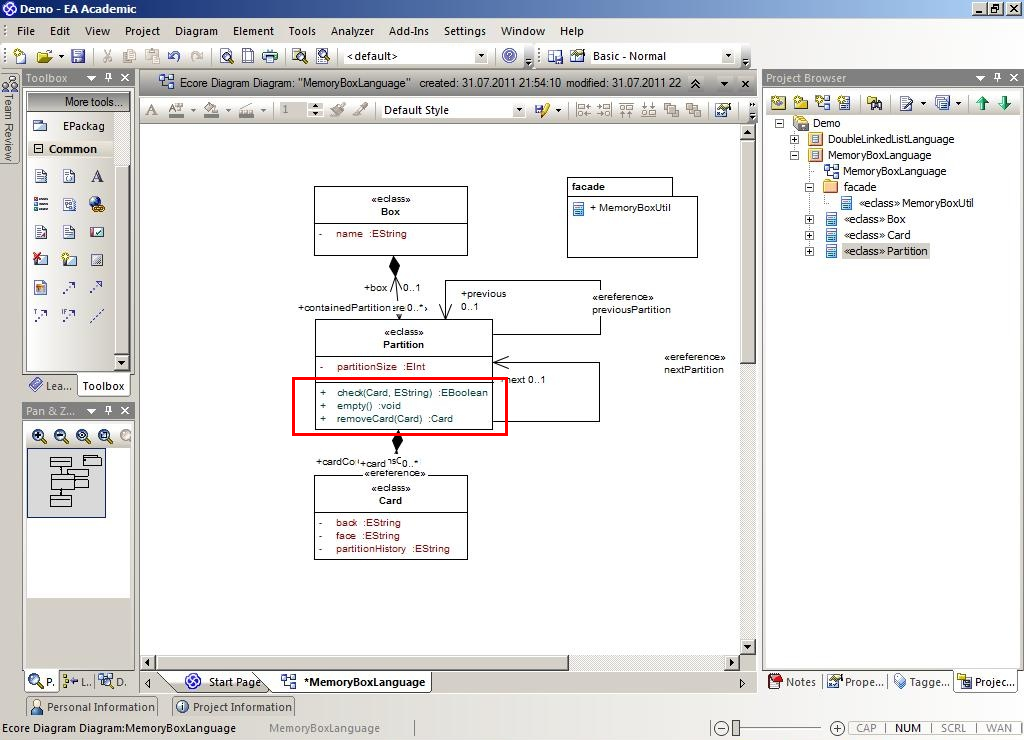
\includegraphics[width=0.6\textwidth]{pics/memBoxBilder/memBox40}
	\caption{Activating the validation output window}
	\label{fig:validation_output}
\end{figure}
\FloatBarrier

\item[$\blacktriangleright$] To start the validation choose ``Extensions/\-MOFLON::Ecore Addin/\-Validate all'' in EA (Fig.~\ref{fig:validation_menu}).
If you haven't already made any mistakes while modelling your \texttt{LearningBoxLanguage} in the last chapter, the output should resemble Fig.~\ref{fig:validation_output}, indicating that your metamodels are free of errors (at least according to our validation).

\begin{figure}[htbp]
	\centering
  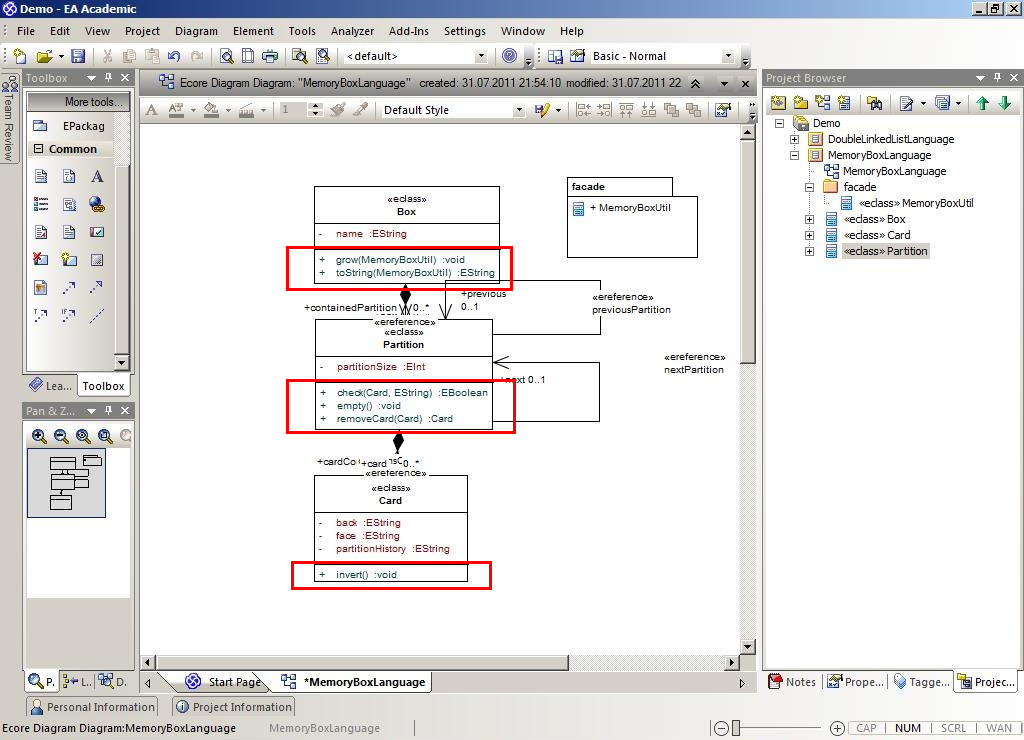
\includegraphics[width=0.6\textwidth]{pics/memBoxBilder/memBox41}
	\caption{Starting the validation}
	\label{fig:validation_menu}
\end{figure}
\FloatBarrier
\end{enumerate}


To get familiar with our validation and quick fix features, let's add two small modelling errors in \texttt{LearningBoxLanguage}.

\begin{enumerate}
\item[$\blacktriangleright$] Create a new class in the \texttt{Learning\-Box\-Language} diagram.
You can retain the default name \texttt{EClass1}.
Let's assume, you wish to delete this class from your metamodel.
\item[$\blacktriangleright$] Select it (\texttt{EClass1}) in the diagram and press the \texttt{Delete} button.
Note that \texttt{EClass1} still exists in the project browser (and thus in your metamodel) and that you have one new \texttt{Information} message in the validation output (Fig.~\ref{fig:validation_information}).

\begin{figure}[htbp]
	\centering
  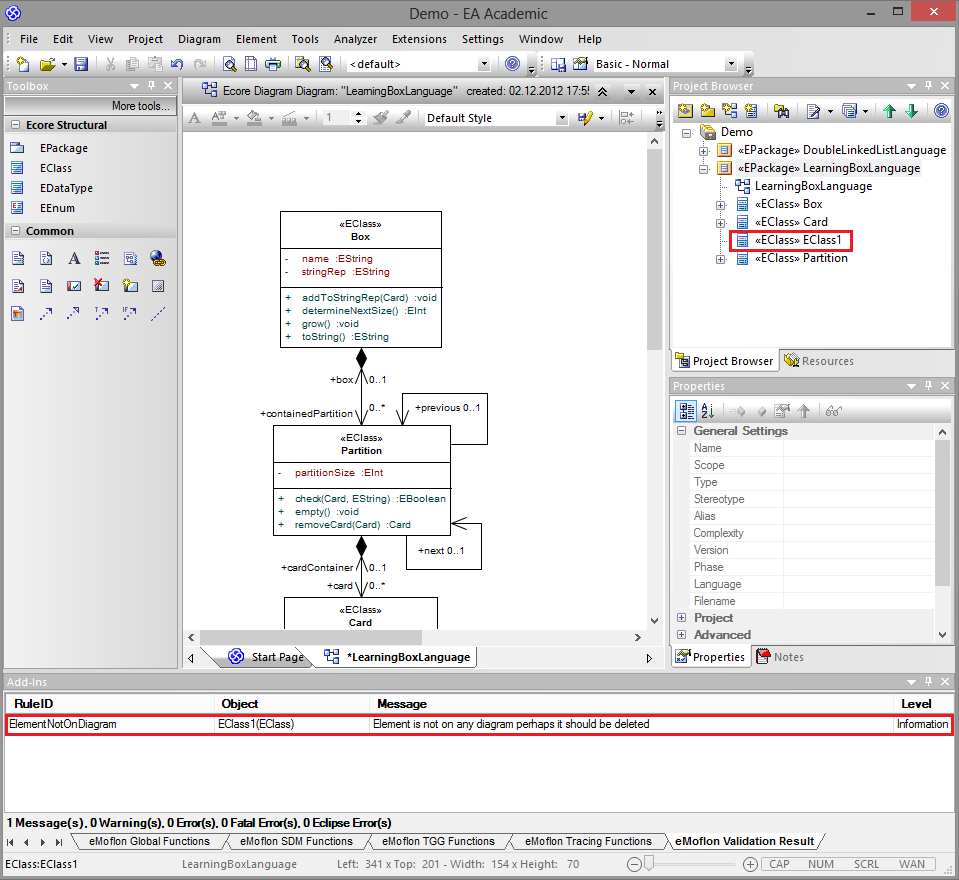
\includegraphics[width=0.7\textwidth]{pics/memBoxBilder/memBox43}
	\caption{Output indicating that an element is present in the metamodel, which is not in any diagram and should probably be deleted completely}
	\label{fig:validation_information}
\end{figure}

The message informs you that \texttt{EClass1} is not on any diagram, and as it is still in the model, that this could be a mistake.
Just pressing the \texttt{Delete} button is apparently not the proper way of \emph{deleting} \texttt{EClass1} from the metamodel and only removes it from the current diagram.
Deleting elements properly and other EA specific aspects are discussed in detail in Chapter~\ref{chap:Tips and Tricks}.


\item[$\blacktriangleright$] To navigate to the problematic element click once on the information message in the output window.
EA should navigate automatically to \texttt{EClass1} and highlight it in the project browser.
\item[$\blacktriangleright$] To check if there are any quick fixes available, double click the information message to invoke the quick fix dialogue.
In this case, there is one quick fix which suggests simply deleting the element from the model (Fig.~\ref{fig:quick-fix1}) as this is probably what was intended.
\item[$\blacktriangleright$] Click \texttt{OK} and \texttt{EClass1} will be deleted correctly from your model.
Your metamodel should now be error-free again as indicated by the validation output window.

\begin{figure}[htbp]
	\centering
  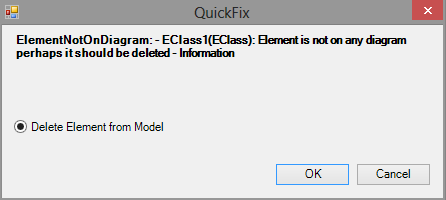
\includegraphics[width=0.55\textwidth]{pics/memBoxBilder/memBox45}
	\caption{Quick fix for elements that are not on any diagram}
	\label{fig:quick-fix1}
\end{figure}
\FloatBarrier

\item[$\blacktriangleright$] To make an error that leads to a more critical message than ``information'',
double click the navigable reference end \texttt{previous} of the class \texttt{Partition}, and delete its role name as depicted in Fig.~\ref{fig:delete-role-name}.
Affirm with \texttt{OK}.

You should now see a new \texttt{Fatal Error} in the validation output, stating that a navigable end \emph{must} have a role name (Fig.~\ref{fig:fatal-error}).
As navigable references are mapped to data members in a Java class, omitting the name of a navigable reference makes code generation impossible (data members, i.e., class variables must have a name).

\begin{figure}[htbp]
    \centering
  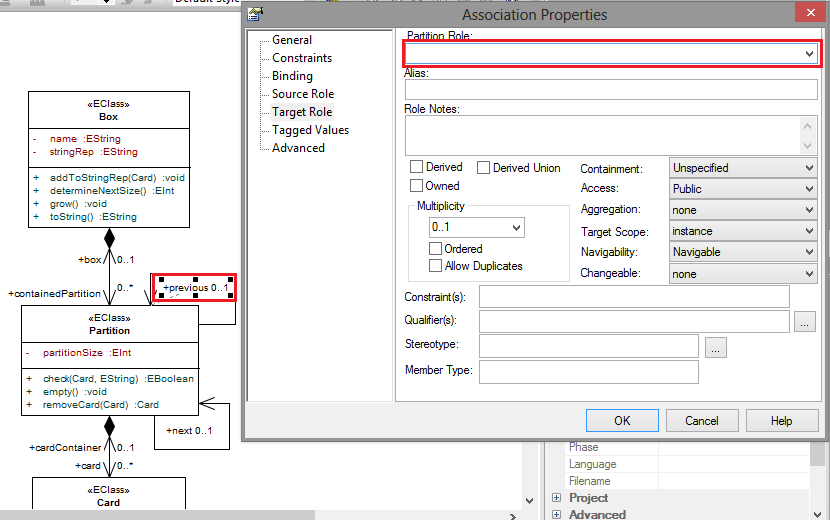
\includegraphics[width=0.85\textwidth]{pics/memBoxBilder/memBox46}
    \caption{Deleting a navigable role name of a reference}
    \label{fig:delete-role-name}
\end{figure}

\item[$\blacktriangleright$] As before, clicking the error message selects the problematic connector in the diagram, and double clicking reveals that there are no quick fixes for this problem (Fig.~\ref{fig:fatal-error}).
\item[$\blacktriangleright$] Correct your metamodel manually by setting the name of the navigable reference back to \texttt{previous}.
\clearpage
\item[$\blacktriangleright$] Ensure that your metamodel closely resembles Fig.~\ref{fig:metamodel_complete} again, and that there are no error messages before you proceed with the rest of the chapter.

\begin{figure}[htbp]
	\centering
  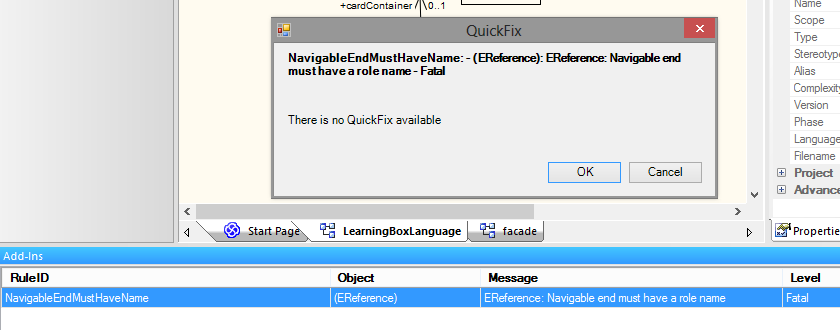
\includegraphics[width=0.7\textwidth]{pics/memBoxBilder/memBox47}
	\caption{Fatal Error after deleting a navigable role name}
	\label{fig:fatal-error}
\end{figure}
\end{enumerate}

As you've probably already noticed, we distinguish between five different types of validation messages:
\begin{description}
  \item[Information:]~\\
  This is only a hint for the user and can be safely ignored if you know what you're doing.
  Export and code generation should be possible, but certain naming/modelling conventions are violated, or a problematic situation has been detected.
  \item[Warning:]~\\ Export and code generation is possible, but only with defaults and automatic corrections applied by the code generator.
  As this might not be what the user wants, such cases are flagged as warnings (e.g., omitting the multiplicity at references which is automatically set by the code generator to 1).
  Being as explicit as possible is often better than relying on defaults.
  \item[Error:]~\\ Although the metamodel can be exported from EA, it is not Ecore conform and code generation will not be possible.
  \item[Fatal Error:]~\\ The metamodel cannot be exported as required information such as names or classifiers of model elements are incorrectly set or missing.
  \item[Eclipse Error:]~\\ Error messages produced by our Eclipse plugin after an unsuccessful attempt to generate code.
  This is currently not actively used.
   %This will be discussed in detail in Sect~\ref{par:validation_in_eclipse}.

\end{description}